\section{nano}

\noindent
\cmd{nano} -- текстовый редактор. Чтобы создать новый файл с именем \argum{file} или открыть существующий в режиме редактирования, необходимо выполнить команду \footnote{если параметр \argum{file} не указывать, то откроется редактор с пустым документом}:

\begin{lstlisting}
	
	$ nano file
	
\end{lstlisting}	

После открытия редактора \cmd{nano} \ref{fig:nano}, внизу можно увидеть следующие подсказками: \verb|^|\textbf{X} Exit, \verb|^|\textbf{G} Help и т.д. В *nix системах сочетения нажатия клавиши \keys{Ctrl} с нажатием другой клавиши обозначается, как символ \verb|^| и далее название клавиши, так нажатие сочетания клавиш \keys{Ctrl + X} и \keys{Ctrl + C} обозначаются, как \verb|^|\textbf{X} и \verb|^|\textbf{C} соответственно.

\begin{figure}[h]
\centering
	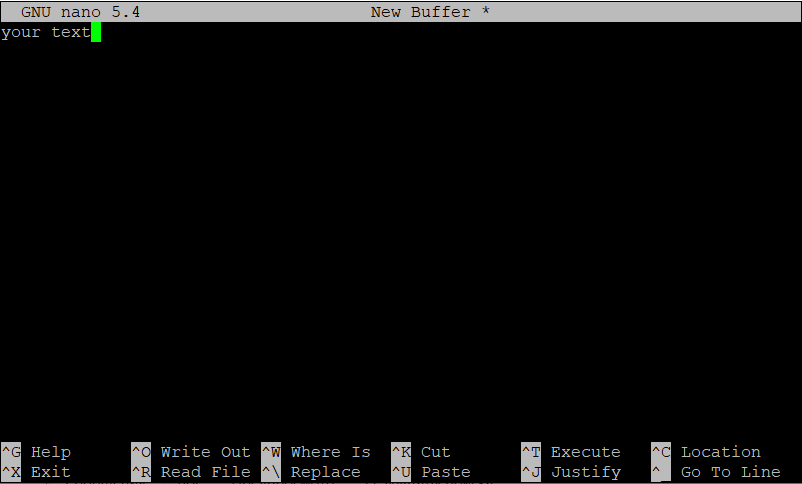
\includegraphics[width=\textwidth]{img/ch1/nano.png}
	\caption{Редактор \cmd{nano} после открытия}
	\label{fig:nano}
\end{figure}

Так же в \cmd{nano} можно открыть более одного файла одновременно, например:
\begin{lstlisting}
	
	$ nano file1 file2 file3
	
\end{lstlisting}	

В результате будут открыты файлы \argum{file1}, \argum{file2} и \argum{file3} в так называемый \textit{буфферах} (экраны, между которыми можно переключаться сочетаниями клавиш \keys{ Atl + > } и \keys{ Atl + < }). Так же можно набор файлов по маске, например:
\begin{lstlisting}
	
	$ nano *.log
	
\end{lstlisting}	

\noindent
\keys{ Ctrl + X } -- закрыть текущий буффер и выйти из \cmd{nano}\\
\keys{ Ctrl + O } -- сохранить изменение текущего буффера в файл\\
\keys{ Ctrl + R } -- открыть файл в текущем буфере\\
(\keys{ Ctrl + R })  + (\keys{ Atl + F }) -- открыть файл в новом буфере\\
(\keys{ Ctrl + R })  + (\keys{ Atl + F }) + (\keys{ Enter }) -- создать новый буффер\\


\subsection*{Редактирование}
\noindent
\keys{ Atl + A }/\keys{ Atl + 6 } -- выделить текст с текущей позиции курсора или отменить выделение\\
\keys{ Ctrl + 6 } -- скопировать выделенный текст\\
\keys{ Ctrl + K } -- вырезать текущую строку или выделенный текст в буфер обмена\\
\keys{ Ctrl + U } -- вставить содержимое буфера обмена в текущую позицию курсора\\
\keys{ Atl + M } -- вырезать от позиции курсора до конца файла\\
\keys{ Ctrl + D } -- удалить символ справа от курсора\\
\keys{ Ctrl + H } -- удалить символ слева от курсора\\
\keys{ Ctrl + M } -- вставить пустую строку\\
\keys{ Atl + R } -- заменить текст или регулярное выражение\\
\keys{ Ctrl + W } -- искать текст или регулярное выражение\\
\keys{ Atl + W } -- повторить последний поиск\\

\subsection*{Навигация}
\noindent
\keys{ PgUp }/\keys{ PgDown } -- пролистать на один экран вверх/вниз\\
\keys{ Ctrl  + }/\keys{ Atl + } -- вперёд/назад  на одно слово\\
\keys{ Atl + E }/\keys{ End } -- в конец текущей строки\\
\keys{ Atl + A }/\keys{ Home } -- в начало текущей строки\\
\keys{ Atl + $\setminus$}/\keys{ / }  -- на первую/последнюю строку файла\\
\keys{ Ctrl + \_ } -- перейти на указанный номер \textbf{строки} или \textbf{строки,позиции}\\

\subsection*{Прочее}
\noindent
\keys{ Atl + C } -- отображение положения курсора включить/отключить\\
\keys{ Ctrl + C } -- показать положение курсора (если в режиме редактирования документа)\\
\keys{ Atl + P } -- отображение пробелов\\
\keys{ Atl + Y } -- подсветка синтаксиса\\
\keys{ Atl + I } -- автоотступы\\
\keys{ Atl + H } -- умная клавиша HOME\\
\keys{ Atl + D } -- подсчитать количество слов, строк и символов в документе\\
\keys{ Atl + M } -- включить/отключить мышку для позиционирования курсора в редакторе\\
\keys{ Atl + N } -- включить/отключить нумерацию строк\\

Открыть файл \argum{file} и перейти к строке \textit{line} и столбцу \textit{col}:
\begin{lstlisting}
	
	$ nano +line,col <file>
	
\end{lstlisting}	

Открыть файл \argum{file} с нумерацией строк:
\begin{lstlisting}
	
	$ nano -l <file>
	
\end{lstlisting}	

Двойное нажатие \keys{Esc}, а затем ввод \textbf{трёхзначного числа} от \textbf{000} до \textbf{255} вставит символ с соответствующим ему hex-кодом.

Открыть файл \argum{file} предварительно сохранив его резервную копию:
\begin{lstlisting}
	
	$ nano -B <file>
	
\end{lstlisting}	

Чтобы указать директорию для сохранения резервных копий редактируемого файла или файлов, используется опция -C:
\begin{lstlisting}
	
	$ nano -BC <dir> <file>
	
\end{lstlisting}	


Открыть файл \argum{file} только для чтения используется ключ -v:
\begin{lstlisting}
	
	$ nano -v <file>
	
\end{lstlisting}	
